\section{Polynomial Decomposition}
This approach is based on the simple computation of the Riemann-Liouville integral for real polynomials:
\begin{equation}
  J^{\alpha}\left(t^{\beta}\right)=\dfrac{\Gamma(\beta+1)}{\Gamma(\alpha+\beta+1)}t^{\alpha+\beta},\quad \alpha>0,\,\beta\in\mathbb{R}
\end{equation}
The main idea is to convert the right-hand side of the approximation with decomposition into polynomials, using polynomial interpolation techniques. This method is useful for non-chaotic fractional dynamic systems or chaotic ones for small time frames.

In order to validate the method, we present three different examples applying the depicted method.

Consider the following multi-term nonlinear fractional differential equation
\begin{equation}\label{ivp:pDeco}
    \begin{cases}
        y'''(t)+\mathcal{D}_c^{5/2}y(t)+y^2(t)=t^4&\\
        y(0)=y'(0)=0,\,y''(0)=2
    \end{cases}
\end{equation}
The exact solution to this FDE is $y(t)=t^2$ \cite{saadatmandi2010new}. The polynomial decomposition was applied and compared with the ABM method (figure \ref{fig:pDeco_exact}).

\begin{figure}
    \centering
    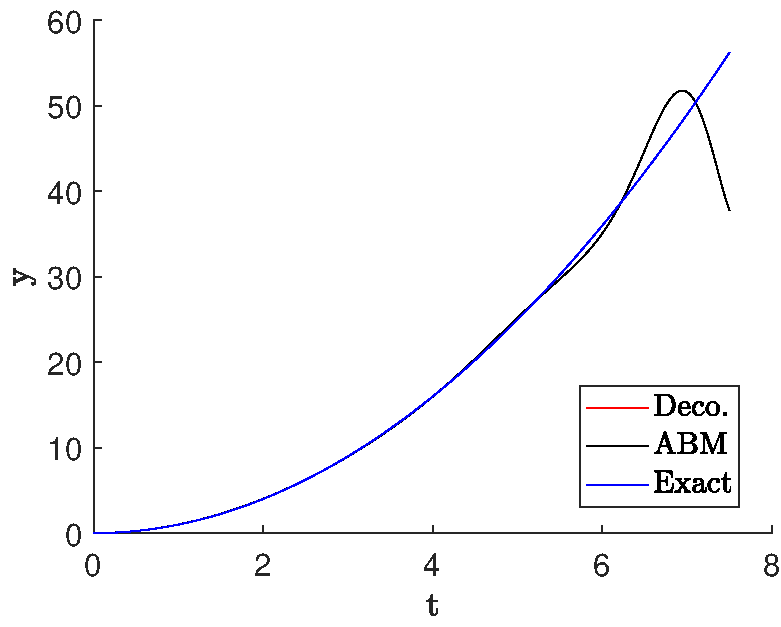
\includegraphics[scale=.5]{files/ABM-vs-Deco-Exact.pdf}
    \caption{Approximate solution to problem \ref{ivp:pDeco} using ABM and polynomial decomposition.}
    \label{fig:pDeco_exact}
\end{figure}
